% Wavelet Multiresolution Analysis (MRA) — Filter bank decomposition
\documentclass[tikz,border=10pt]{standalone}
\usepackage{tikz}
\usepackage{amsmath, amssymb}
\usetikzlibrary{arrows.meta, positioning, calc, decorations.pathreplacing}

% GDL color palette
\definecolor{gdlblue}{RGB}{41, 98, 168}
\definecolor{gdlred}{RGB}{191, 49, 49}
\definecolor{gdlgreen}{RGB}{30, 130, 76}
\definecolor{gdlorange}{RGB}{217, 130, 30}
\definecolor{gdlpurple}{RGB}{118, 56, 138}
\definecolor{gdlgray}{RGB}{140, 140, 140}
\definecolor{gdlyellow}{RGB}{190, 140, 10}

\begin{document}
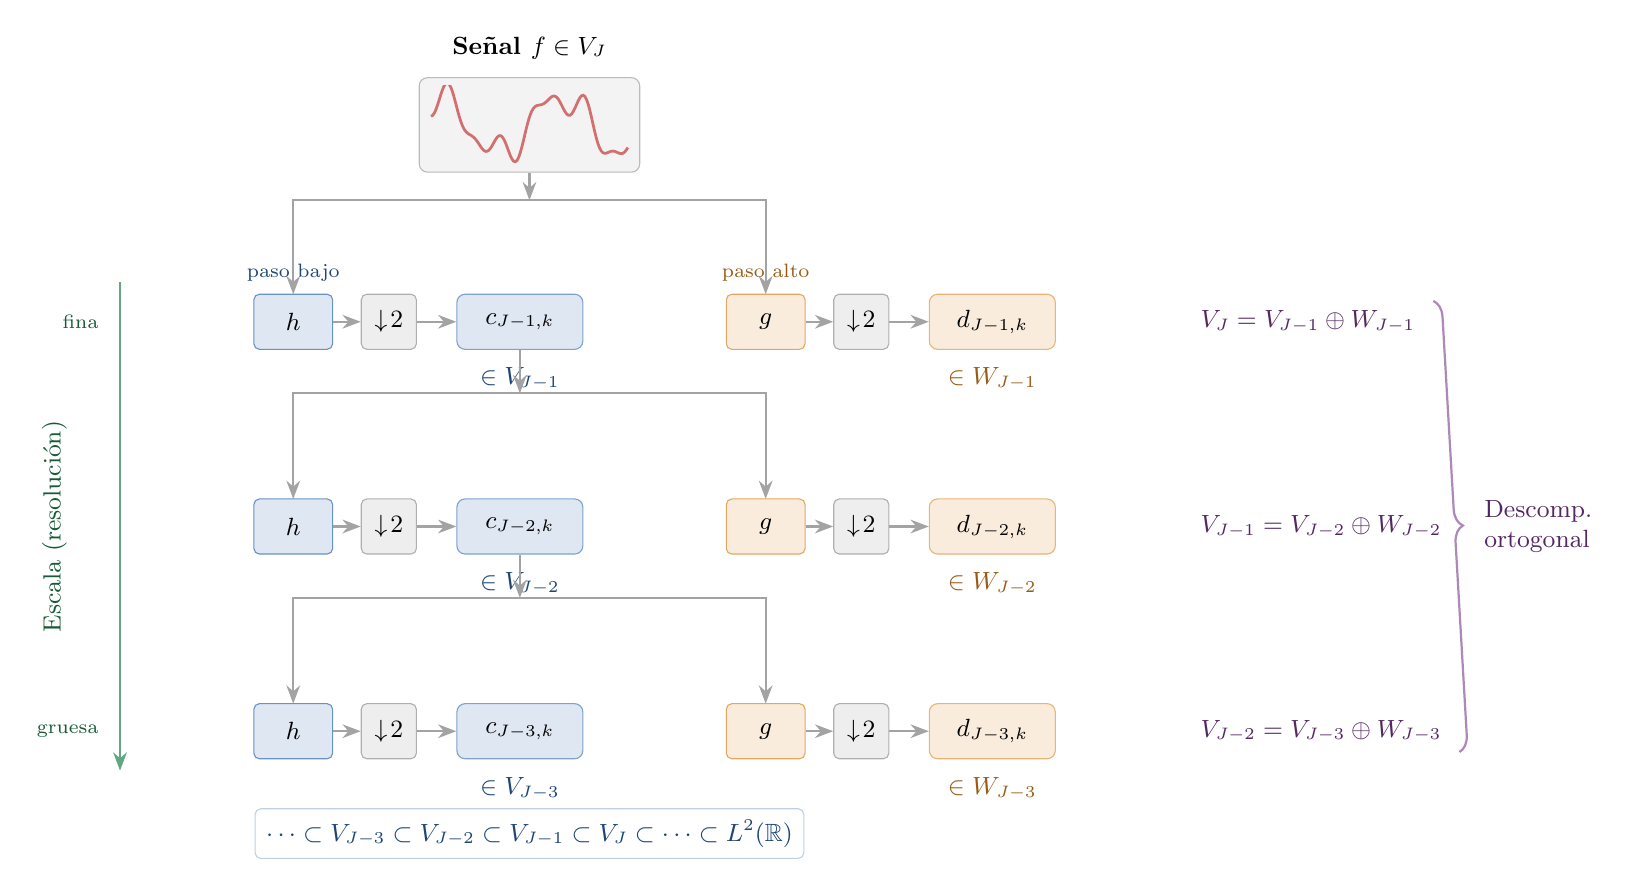
\begin{tikzpicture}[
  >=Stealth,
  filter/.style={
    draw=#1!70, fill=#1!15, minimum width=1.0cm, minimum height=0.7cm,
    font=\small, rounded corners=2pt, inner sep=2pt
  },
  downsample/.style={
    draw=gdlgray!70, fill=gdlgray!15, minimum width=0.7cm, minimum height=0.7cm,
    font=\small, rounded corners=2pt, inner sep=2pt
  },
  coeff/.style={
    draw=#1!60, fill=#1!15, minimum width=1.6cm, minimum height=0.7cm,
    font=\small, rounded corners=3pt, inner sep=3pt
  },
  arrowline/.style={->, gdlgray!80, thick},
]

% Layout constants
\def\rowsep{2.6}       % vertical spacing between decomposition levels
\def\collow{-1.8}      % x-center of low-pass branch
\def\colhigh{4.2}      % x-center of high-pass branch

% ===================================================================
% TOP: Input signal f
% ===================================================================

\node[draw=gdlgray!60, fill=gdlgray!10, minimum width=2.8cm, minimum height=1.2cm,
      rounded corners=3pt] (fbox) at (1.2, 0) {};

% Draw a composite waveform inside the box
\begin{scope}
  \clip ([xshift=3pt, yshift=3pt]fbox.south west) rectangle ([xshift=-3pt, yshift=-3pt]fbox.north east);
  \draw[gdlred!70, line width=1.0pt]
    plot[domain=-1.25:1.25, samples=120, smooth]
    ({1.2 + \x}, {0.35*sin(4*\x r) + 0.15*sin(11*\x r) + 0.1*cos(18*\x r)});
\end{scope}

\node[above=3pt of fbox, font=\bfseries\small, text=black] {Se\~nal $f \in V_J$};

% ===================================================================
% LEVEL 1:  J -> J-1
% ===================================================================
\def\lva{-2.5}

% Split arrow from signal
\draw[arrowline] (fbox.south) -- ++(0, -0.35) coordinate (splitA);
\draw[gdlgray!80, thick] (splitA) -| (\collow, {\lva + 0.6});
\draw[arrowline] (\collow, {\lva + 0.6}) -- (\collow, {\lva + 0.35});
\draw[gdlgray!80, thick] (splitA) -| (\colhigh, {\lva + 0.6});
\draw[arrowline] (\colhigh, {\lva + 0.6}) -- (\colhigh, {\lva + 0.35});

% Low-pass filter h
\node[filter=gdlblue] (hA) at (\collow, \lva) {$h$};
\node[above=1pt of hA, font=\scriptsize, text=gdlblue!70!black] {paso bajo};
\node[downsample, right=0.35cm of hA] (dsA) {$\downarrow\!2$};
\draw[arrowline] (hA) -- (dsA);

% Approximation output c_{J-1}
\node[coeff=gdlblue, right=0.5cm of dsA] (cJ1) {$c_{J-1,k}$};
\draw[arrowline] (dsA) -- (cJ1);
\node[below=3pt of cJ1, font=\small, text=gdlblue!70!black] {$\in V_{J-1}$};

% High-pass filter g
\node[filter=gdlorange] (gA) at (\colhigh, \lva) {$g$};
\node[above=1pt of gA, font=\scriptsize, text=gdlorange!70!black] {paso alto};
\node[downsample, right=0.35cm of gA] (dsAgA) {$\downarrow\!2$};
\draw[arrowline] (gA) -- (dsAgA);

% Detail output d_{J-1}
\node[coeff=gdlorange, right=0.5cm of dsAgA] (dJ1) {$d_{J-1,k}$};
\draw[arrowline] (dsAgA) -- (dJ1);
\node[below=3pt of dJ1, font=\small, text=gdlorange!70!black] {$\in W_{J-1}$};

% ===================================================================
% LEVEL 2:  J-1 -> J-2
% ===================================================================
\pgfmathsetmacro{\lvb}{\lva - \rowsep}

% Split arrow from c_{J-1}
\draw[arrowline] (cJ1.south) -- ++(0, -0.55) coordinate (splitB);
\draw[gdlgray!80, thick] (splitB) -| (\collow, {\lvb + 0.6});
\draw[arrowline] (\collow, {\lvb + 0.6}) -- (\collow, {\lvb + 0.35});
\draw[gdlgray!80, thick] (splitB) -| (\colhigh, {\lvb + 0.6});
\draw[arrowline] (\colhigh, {\lvb + 0.6}) -- (\colhigh, {\lvb + 0.35});

% Low-pass
\node[filter=gdlblue] (hB) at (\collow, \lvb) {$h$};
\node[downsample, right=0.35cm of hB] (dsB) {$\downarrow\!2$};
\draw[arrowline] (hB) -- (dsB);
\node[coeff=gdlblue, right=0.5cm of dsB] (cJ2) {$c_{J-2,k}$};
\draw[arrowline] (dsB) -- (cJ2);
\node[below=3pt of cJ2, font=\small, text=gdlblue!70!black] {$\in V_{J-2}$};

% High-pass
\node[filter=gdlorange] (gB) at (\colhigh, \lvb) {$g$};
\node[downsample, right=0.35cm of gB] (dsBgB) {$\downarrow\!2$};
\draw[arrowline] (gB) -- (dsBgB);
\node[coeff=gdlorange, right=0.5cm of dsBgB] (dJ2) {$d_{J-2,k}$};
\draw[arrowline] (dsBgB) -- (dJ2);
\node[below=3pt of dJ2, font=\small, text=gdlorange!70!black] {$\in W_{J-2}$};

% ===================================================================
% LEVEL 3:  J-2 -> J-3
% ===================================================================
\pgfmathsetmacro{\lvc}{\lvb - \rowsep}

% Split arrow from c_{J-2}
\draw[arrowline] (cJ2.south) -- ++(0, -0.55) coordinate (splitC);
\draw[gdlgray!80, thick] (splitC) -| (\collow, {\lvc + 0.6});
\draw[arrowline] (\collow, {\lvc + 0.6}) -- (\collow, {\lvc + 0.35});
\draw[gdlgray!80, thick] (splitC) -| (\colhigh, {\lvc + 0.6});
\draw[arrowline] (\colhigh, {\lvc + 0.6}) -- (\colhigh, {\lvc + 0.35});

% Low-pass
\node[filter=gdlblue] (hC) at (\collow, \lvc) {$h$};
\node[downsample, right=0.35cm of hC] (dsC) {$\downarrow\!2$};
\draw[arrowline] (hC) -- (dsC);
\node[coeff=gdlblue, right=0.5cm of dsC] (cJ3) {$c_{J-3,k}$};
\draw[arrowline] (dsC) -- (cJ3);
\node[below=3pt of cJ3, font=\small, text=gdlblue!70!black] {$\in V_{J-3}$};

% High-pass
\node[filter=gdlorange] (gC) at (\colhigh, \lvc) {$g$};
\node[downsample, right=0.35cm of gC] (dsCgC) {$\downarrow\!2$};
\draw[arrowline] (gC) -- (dsCgC);
\node[coeff=gdlorange, right=0.5cm of dsCgC] (dJ3) {$d_{J-3,k}$};
\draw[arrowline] (dsCgC) -- (dJ3);
\node[below=3pt of dJ3, font=\small, text=gdlorange!70!black] {$\in W_{J-3}$};

% ===================================================================
% RIGHT PANEL: Orthogonal decomposition equations
% ===================================================================

% Position equations well clear of the detail boxes
\def\eqx{9.6}

\node[font=\small, text=gdlpurple!70!black, anchor=west] (eq1) at (\eqx, \lva)
  {$V_{J} = V_{J-1} \oplus W_{J-1}$};
\node[font=\small, text=gdlpurple!70!black, anchor=west] (eq2) at (\eqx, \lvb)
  {$V_{J-1} = V_{J-2} \oplus W_{J-2}$};
\node[font=\small, text=gdlpurple!70!black, anchor=west] (eq3) at (\eqx, \lvc)
  {$V_{J-2} = V_{J-3} \oplus W_{J-3}$};

% Brace grouping the three equations (on the right side)
\draw[gdlpurple!60, thick, decorate, decoration={brace, amplitude=6pt}]
  ([xshift=3pt]eq1.north east) -- ([xshift=3pt]eq3.south east)
  node[midway, right=10pt, font=\small, text=gdlpurple!70!black, align=left]
  {Descomp.\\ortogonal};

% ===================================================================
% LEFT PANEL: Scale arrow
% ===================================================================
\def\arrowx{-4.0}

\draw[gdlgreen!70, thick, ->] (\arrowx, {\lva + 0.5}) -- (\arrowx, {\lvc - 0.5});
\node[font=\scriptsize, text=gdlgreen!70!black, anchor=east] at ({\arrowx - 0.15}, \lva) {fina};
\node[font=\scriptsize, text=gdlgreen!70!black, anchor=east] at ({\arrowx - 0.15}, \lvc) {gruesa};
\node[font=\small, text=gdlgreen!70!black, rotate=90, anchor=south] at ({\arrowx - 0.55}, {\lvb})
  {Escala (resoluci\'on)};

% ===================================================================
% BOTTOM: Nesting of approximation spaces
% ===================================================================
\pgfmathsetmacro{\nesty}{\lvc - 1.3}
\node[font=\small, text=gdlblue!70!black, fill=white, inner sep=4pt,
      rounded corners=2pt, draw=gdlblue!30] at (1.2, \nesty)
  {$\cdots \subset V_{J-3} \subset V_{J-2} \subset V_{J-1} \subset V_J
   \subset \cdots \subset L^2(\mathbb{R})$};

\end{tikzpicture}
\end{document}
